\chapter{Sample figures and tables}\label{Ch:figures}

\section{Figures}

% Note that the label follows the caption.
\begin{figure}[ht]
\begin{center}
\includegraphics[width=0.3\textwidth]{Graphics/ipamlogo.eps}
\end{center}
\caption{A sample \textsc{eps} figure with a caption.}\label{FIGURE:IPAM-logo-eps}
\end{figure} 


\subsubsection{Formats accepted by {\LaTeX}}
This version of the  RIPS {\LaTeX } template can be used to produce a pdf of your report using several different typesetters, including \texttt{pcTeX} and other options available on the IPAM network.
All of these will accept figures in the encapsulated postscript (\textsc{eps}) format providing you incorporate the appropriate \emph{packages} in the \emph{preamble} of your {\LaTeX] code.%%
\footnote{
The RIPS reports template devotes a section of the preamble to a method for ensuring that your chosen typesetter will be able to utilize eps files. 
This is one of several options for affecting formats that you will find explained by comments in the preamble.
For a good source for general information on incorporating graphics in {\LaTeX}, see
\texttt{http://amath.colorado.edu/documentation/LaTeX/reference/figures.html}.
}%% 
The LaTeX code for Figure \ref{FIGURE:IPAM-logo-eps} shows how to emplace, label and reference it.
You may have to convert the format for your figure.
But beware, incorporating graphics in {\LaTeX} can be quirky and require special attention and work-arounds.%%
\footnote{There is a simple way to make format conversions that works in some cases.
Click on the file in its current format, then when the graphic appears on your screen use ``save as'' to write the graphic in a format you select from the given options.
See Chapter 7 for more suggestions.}

\subsubsection{Creating figures with {\textsc{Matlab}}}
Here's a sample code, describing how to create a figure in \textsc{Matlab} and export it as \textsc{eps}.

\begin{verbatim}
%% Shows how to make a MATLAB figure

%% create a vector of N points between a and b
a=-1.2; b = -a; N = 100; X=linspace(a, b, N);

Y = X.^3 - X; % a function of X

figure(1); clf; % pop up a figure, clean it

H = axes; set(H, 'fontsize', 20); % set the font

plot(X, Y, 'color', 'blue', 'linewidth', 2); % plot

axis([a, b, -0.6, 0.6]); % the viewable box

saveas(gcf, 'MyPicture.eps', 'psc2'); % save the picture in color
\end{verbatim}

\begin{figure}[h]
\begin{center}
\includegraphics[clip, width=0.4\textwidth]{Graphics/MatlabPicture.eps}
\caption[A sample figure created as an \texttt{eps} file by \textsc{Matlab}]{A sample figure created as an \texttt{eps} file by \textsc{Matlab}.
To see an example of quirky treatment, compare this figure when you typeset the report template with \textsc{PCTeX} and pdf{\LaTeX}.}\label{FIGURE:fromMatlab}
\end{center}
\end{figure}

The source code for Figure \ref{FIGURE:fromInkScape} is available in the sample RIPS report directory. 
The {\LaTeX}code for incorporating this figure in the report template is:

\vspace{8pt}
\begin{quote} 
{\tt $\backslash$begin\{figure\}[h]\\
{\tt $\backslash$begin\{center\}} \\
{\tt $\backslash$includegraphics[clip, width=0.4$\backslash$textwidth]{Graphics/MatlabPicture.eps}} \\
{\tt $\backslash$caption\{A sample figure created with $\backslash$textsc\{Matlab\}.\}}$\backslash$label{<name of label}}  \\
{\tt $\backslash$end\{center\}} \\
{\tt $\backslash$end\{figure\}}
\end{quote}

Beware: your label identifier should always follow the caption statement.
You can place it higher up without crashing the {\LaTeX} compiler, but doing so can result in an erroneous enumeration for the label in your text.

\subsubsection{Software for drawing diagrams}

There exist many programs for drawing figures and diagrams.
If you have a preferred system, please let the RIPS director know about it.
Maybe it should be referenced here.
The following two were recommended by Academic Mentors:

\textsc{PSTricks} is a powerful system for designing and incorporating fine mathematical graphics into {\TeX} and {\LaTeX} documents.
Be aware that it works directly with inline code for some {\LaTeX} typesetters but  requires special handling for pdf{\LaTeX}.  
See Figure \ref{FIGURE:fromPSTricks}.


\begin{figure}[h]
\begin{center}
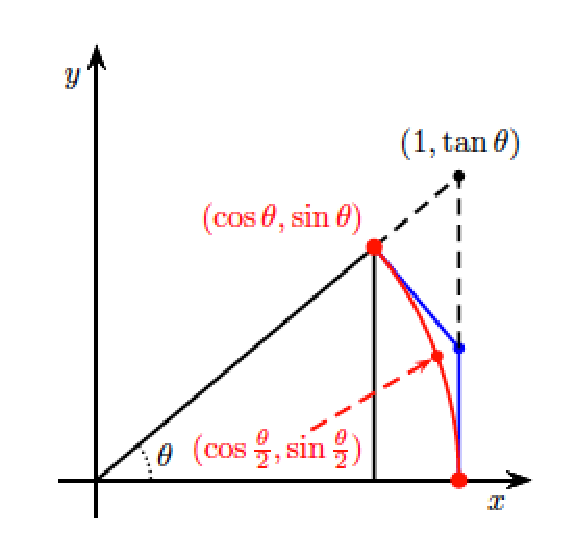
\includegraphics[clip, width=0.4\textwidth]{Graphics/SineTheta5-CS.eps}
\caption[A sample figure created as an \texttt{eps} file by \textsc{Matlab}]{PSTricks code for this figure is in the ``Graphics'' folder for the {\LaTeX} template.
The code was run using Xe{\LaTeX} and the resulting \texttt{pdf} file was converted to an \texttt{eps} file.}\label{FIGURE:fromPSTricks}
\end{center}
\end{figure}


\emph{Inkscape} is free and of high quality;
with this program, you should always keep the figures in Inkscape's native \textsc{svg} format,
and save them as \textsc{eps} only in order to view them in {\LaTeX}.


\begin{figure}[ht]
\label{fig2}
\begin{center}
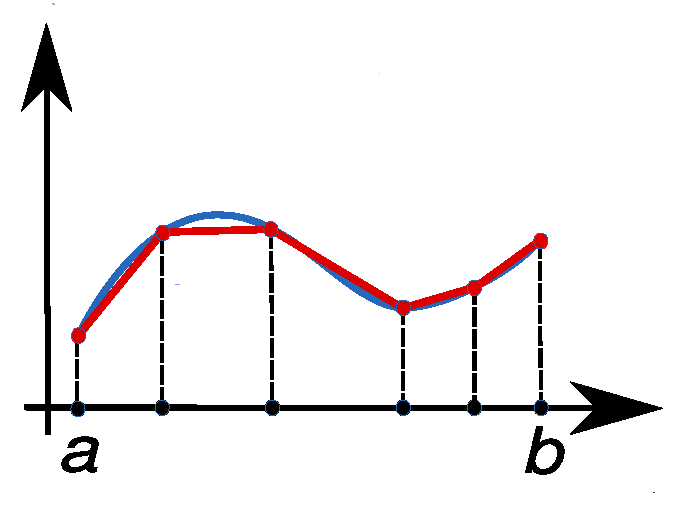
\includegraphics[width=0.4\textwidth]{Graphics/Figure1.eps}

\includegraphics[width=0.309\textwidth]{Graphics/Figure2.eps}
\end{center}
\caption{A couple of figures drawn with Inkscape.}\label{FIGURE:fromInkScape}
\end{figure}

The two adjacent graphics in Figure \ref{FIGURE:fromInkScape} were created with Inkscape and exported to \textsc{eps}.
The figures in the original \textsc{svg} format are available in the report directory.
Note that the convention for punctuating a figure caption or table caption is pretty loose.
If an initial phrase is followed by a complete sentence, the phrase as well as any complete sentence should be ended with a period.
For consistency, it is \textsc{ok} to end all captions with a period even if a caption is just a phrase, as are all three captions illustrated here.

\section{Tables}

\noindent The next example is a simple table: Table \ref{TABLE:Simple}.
The {\LaTeX} code for it is presented after the table. 

% Note that the label follows the caption.
\begin{table}[h]
\begin{center}
  \begin{tabular}{|lcc|}
    \hline
    Date & High & Low\\ \hline
    1-Jul & 40 & 12\\
    2-Jul & 37 & 14\\
    3-Jul & 35 & 20\\ \hline
  \end{tabular}
\end{center}
\caption{A simple table showing fictional data.}\label{TABLE:Simple}
\end{table}

Look at the following source code for Table \ref{TABLE:Simple}, and note particularly how it is labeled.
The references to it in the two preceding sentencs were created by incorporating the label in the {\LaTeX} code 
(``\verb+Table \ref{TABLE:Simple}+'') used for creating this chapter.
Tables are labeled and referenced in a way similar to figures.

\begin{verbatim}
% Note that the label follows the caption.
\begin{table}[h]
\begin{center}
  \begin{tabular}{|lcc|}
    \hline
    Date & High & Low\\ \hline
    1-Jul & 40 & 12\\
    2-Jul & 37 & 14\\
    3-Jul & 35 & 20\\ \hline
  \end{tabular}
\end{center}
\caption{A sample table showing fictional data.}\label{TABLE:Simple}
\end{table}
\end{verbatim}

The next example, Table \ref{TABLE:SplitText}, illustrates a table in which column widths are specified by parameters in order to force long text to be spread over more than one line: 

\begin{table}[h]
\begin{center}
\begin{tabular}{|p{1in}|p{2in}|} \hline
Betty & Betty has a story to tell. \\ \hline
Bob   & Bob has a longer story to tell. \\ \hline
Bill  & Bill has a very much longer and far more dramatic story to tell. \\ \hline
\end{tabular}
\caption{A sample table with split lines of text.}\label{TABLE:SplitText}
\end{center}
\end{table}

\noindent Here's the code for Table \ref{TABLE:SplitText}:

\begin{verbatim}
\begin{table}[h]
\begin{center}
\begin{tabular}{|p{1in}|p{2in}|} \hline
Betty & Betty has a story to tell. \\ \hline
Bob   & Bob has a longer story to tell. \\ \hline
Bill  & Bill has a very much longer and far more dramatic story to tell. \\ \hline
\end{tabular}
\caption{A sample table with split lines of text.}\label{TABLE:SplitText}
\end{center}
\end{table}
\end{verbatim}

\subsubsection{Style tips about figures and tables}
You should always make sure that your figures are easy to see, so for example, make sure that any curves are not too thin or text is not too small.
And don't forget to include axis labels with units specified.

Your figures should look good both in color and as black-and-white, since for presentations you will most likely want figures in color, while in a printed report all the figures will usually be printed in black-and-white (and then, what looks very clear and pretty on your screen may appear as a dark region on paper).

Good captions greatly improve the usefulness of figures and tables.

But no matter how well a caption describes a figure or table, you should always reference it and explain it in your text.
You may feel you are being redundant, but your readers won't think so:
a picture with a good description is worth a thousand words, and a picture without a description in the text is left dangling.

\section{Picking nits}
Notice that in this sample report, all of the captions for figures and tables are placed below the object, and their labels end with a numbered identifier---e.g., Figure 4.1, Table 4.2---terminated with a colon (``:'') inserted automatically by the {\LaTeX} compiler. 
\emph{The Chicago Manual of Style} specifies the use of a period (``.'') to follow the figure number and a blank space to follow the table number, and \emph{New Hart's Rules} follows both figure and table numbers with a blank space.  
Moreover, \emph{New Hart's Rules} places table captions above the table, rather than beneath.
But here we bow to usage in {Gr\"{a}tzer's} \emph{More Math Into {\LaTeX}}(See Bibliography for references).
In such minutiae it's your choice, but remember, consistency (perhaps a hobgoblin of lesser minds but certainly a ruling passion in typography) is standard practice. 


Another place to be on guard is in referencing, e.g., sections, equations, and lemmas.
Do you capitalize or leave it in lower case: Chapter 1 or chapter 1, Theorem 1 or theorem 1, Lemma 1 or lemma 1?
Of course at sentence heads you have no choice but to capitalize.
When you refer to a figure or a table, you may write, for example, ``Fig. 1'', ``Figure 1'', with or without an initial capital, and write ``Table 1'' or ``table 1''.
Recommended usage for this report is to use proper nouns: whether abreviated or spelled out in full, capitalize the labels.
It's up to you, but be consistent.

You'll think of other things as you go along.
Just consider how it looks on the page, and {\it be consistent throughout your report}.

\endinput

